%--------------------------------------------------------------
% thesis.tex 
%--------------------------------------------------------------
% Corso di Laurea in Informatica 
% - template for the main file of Informatica@Unifi Thesis 
% - based on Classic Thesis Style Copyright (C) 2008 
%   Andr\'e Miede http://www.miede.de   
%--------------------------------------------------------------
\documentclass[twoside,openright,titlepage,fleqn,
	headinclude,12pt,a4paper,BCOR=5mm,footinclude]{scrbook}

\usepackage[nottoc, notlot]{tocbibind}
%--------------------------------------------------------------
% Inputs for the title page 
%--------------------------------------------------------------
\newcommand{\myItalianTitle}{Applicazione di FACPL per la gestione delle policy nei sistemi cloud: un caso di studio concreto con OpenNebula\xspace}
\newcommand{\myEnglishTitle}{Applying FACPL to Policy Management in Cloud Systems: A Practical Case Study with OpenNebula\xspace}
% use the right myDegree option
\newcommand{\myDegree}{Corso di Laurea in Informatica\xspace}
%\newcommand{\myDegree}{Corso di Laurea Magistrale in Informatica\xspace}
\newcommand{\myName}{Matteo Monicolini\xspace}
\newcommand{\mySupervisorTitle}{Relatore\xspace}
\newcommand{\mySupervisorName}{\textit{Rosario Pugliese}\xspace} 
\newcommand{\myTime}{Anno Accademico 2023-2024\xspace}
%--------------------------------------------------------------

\usepackage[utf8]{inputenc} 
\usepackage[T1]{fontenc} 

% switch italian and english, depending on the language of the thesis
% this will change the chapter titles
\usepackage[italian]{babel}
%\usepackage[english]{babel}
\usepackage{csquotes}

\usepackage[fleqn]{amsmath}  
\usepackage{ellipsis}
\usepackage{listings}
\usepackage{subfig}
\usepackage{caption}
\usepackage{appendix}
\usepackage{siunitx}
\usepackage[pdftex]{graphicx} 
\graphicspath{{./Figures/}}
 \usepackage[eulerchapternumbers,linedheaders,subfig,beramono,eulermath,
parts,dottedtoc]{classicthesis}

%--------------------------------------------------------------
% Layout setting
%--------------------------------------------------------------
\newlength{\abcd} 
\newcommand{\myfloatalign}{\centering} 
\setlength{\extrarowheight}{3pt} 
\captionsetup{format=hang,font=small}

\usepackage{geometry}
\geometry{
	a4paper,
	ignoremp,
	bindingoffset = 1cm, 
	textwidth     = 13.5cm,
	textheight    = 21.5cm,
	lmargin       = 3.5cm, 
	tmargin       = 4cm    
}

\lstset{
  	frame=tb,
  	aboveskip=3mm,
  	belowskip=3mm,
  	showstringspaces=false,
  	columns=flexible,
  	basicstyle={\footnotesize\ttfamily},
  	breaklines=true,
  	breakatwhitespace=true,
  	tabsize=3,
	escapechar={@+},
	numbers=left,
	float
}
%--------------------------------------------------------------
\begin{document}
\frenchspacing
\raggedbottom
\pagenumbering{roman}
\pagestyle{plain}
%--------------------------------------------------------------
% Frontmatter
%--------------------------------------------------------------
\include{FrontMatter/Titlepage}
\pagestyle{scrheadings}
%--------------------------------------------------------------
% Mainmatter
%--------------------------------------------------------------
\let\origcleardoublepage\cleardoublepage
\let\cleardoublepage\clearpage
\pagenumbering{arabic}
\addtocontents{toc}{\protect\enlargethispage{\baselineskip}}
\addtocontents{toc}{\protect\enlargethispage{\baselineskip}}
\tableofcontents
\phantomsection
\lstlistoflistings
\phantomsection
\listoffigures
\let\cleardoublepage\origcleardoublepage
\cleardoublepage
\thispagestyle{empty}
\begin{flushright}
\null\vspace{\stretch {1}}
%--------------------------------------------------------------
% Citation
%--------------------------------------------------------------
\emph{"Sarà che prendo troppo spesso Trenitalia ma io non credo nelle coincidenze" \break --- Pinguini tattici nucleari "Test di ingresso di medicina"} \vspace{\stretch{2}}\null
\end{flushright}
\cleardoublepage

%--------------------------------------------------------------
% Chapters
%--------------------------------------------------------------
% !TEX root = ../Thesis.tex

\chapter{Introduzione}
In questa tesi si cercherà di dare una risposta al problema della gestione delle policy nei sistemi cloud, con particolare interesse riguardo le politiche di creazione delle virtual machine e di bilanciamento delle risorse. Il linguaggio utilizzato per le policy è FACPL, ancora poco esplorato nonostante i molti vantaggi rispetto alle alternative presenti in letteratura.\par
Il sistema di gestione cloud scelto è OpenNebula, un software completamente open-source che permette di gestire infrastrutture cloud su diversi livelli e integra molti servizi utili per la gestione delle risorse.\par
L'obiettivo finale è quello di fornire un'implementazione concreta di FACPL come gestore di richieste di creazione di virtual machine che sia in grado di funzionare in un ambiente cloud reale su cui è installato OpenNebula. Questo permetterà quindi di decidere le policy con cui si permette a specifici utenti di creare virtual machine su specifici host, così come di bilanciare le risorse tra i vari host o di decidere di spegnere alcune macchine in base a determinate condizioni.\par
L'implementazione sarà corredata con adeguata metodologia di logging delle informazioni e utilizzo delle pratiche di buona programmazione per rendere il codice facilmente mantenibile e ampliabile in futuro.\par
I principali problemi che saranno affrontati e risolti sono quelli scaturiti dalla necessità di far interagire le API di OpenNebula con la struttura fornita da FACPL senza snaturare nessuno dei due progetti in modo anche da dimostrare la facile adattabilità di FACPL. Un'altra questione che verrà trattata sarà inoltre l'integrazione di un software di gestione della build come Maven, con due progetti distribuiti esclusivamente come file .jar.\par
Per concludere verrà fornito uno spunto di web-app da cui sarà possibile provare le funzionalità del progetto sviluppato oltre che partire per una possibile implementazione in un vero server che integra un meccanismo di autenticazione e autorizzazione.\par
Questa tesi spera di mostrare la semplicitià di utilizzo di FACPL e di evidenziare i suoi pro e contro di modo che una persona che intende realizzare un progetto in cui è richiesta la valutazione di policy di accesso, possa scegliere FACPL come linguaggio se fa al caso suo e con la possibilità di avere un'idea su come può essere utilizzato in un caso concreto.
\section{Guida alla lettura}
I capitoli che seguono sono così suddivisi:
\begin{itemize}
    \item \emph{capitolo 2:} introduce i concetti di base su FACPL e OpenNebula, con particolare attenzione alle componenti usate in questa tesi;
    \item \emph{capitolo 3:} descrive nel dettaglio l'implementazione fornita con diverse spiegazioni sulle scelte di design effettuate;
    \item \emph{capitolo 4:} mostra un'esempio di utilizzo dei progetti e delle conseguenze su un sistema cloud reale;
    \item \emph{capitolo 5:} conclude la tesi con un riassunto dei risultati e possibili sviluppi futuri.
\end{itemize}
% !TEX root = ../Thesis.tex

\chapter{Il linguaggio FACPL e il software OpenNebula}
\label{cap:capitolo2}
L'obiettivo di questo capitolo è introdurre i concetti di base del linguaggio FACPL e del software OpenNebula, necessari per comprendere il lavoro svolto in questa tesi. In particolare, sarà discusso il funzionamento del linguaggio FACPL, le sue caratteristiche principali e le motivazioni che hanno portato al suo utilizzo. Successivamente verrà presentato il software OpenNebula, sarà descritta la sua architettura e saranno evidenziate funzionalità ritrovabili all'interno dei progetti descritti nei capitoli successivi, in modo da comprendere come si può adattare ad un sistema di gestione delle policy basato su FACPL.\medbreak
\section{Il linguaggio FACPL}
Il linguaggio FACPL\footnote{\cite{FAPCLTesi}} è stato ideato nel 2012 come risposta alla necessità di sistemi di controllo degli accessi più flessibili e adattabili di quelli già esistenti. In particolar modo il linguaggio viene spesso paragonato con XACML, questo perchè è attualmente il inguaggio più largamente utilizzato per il controllo degli accessi ma anche perchè FACPL è stato sviluppato proprio come risposta ad alcune evidenti problematiche di XACML. Il problema principale che FACPL punta a risolvere è la mancanza di una semantica definita formalmente, il che rende difficile ideare delle tecniche di analisi.\medbreak
\section{Componenti del sistema FACPL}
\label{sec:componentiFACPL}
FACPL trae larga ispirazione da XACML, in particolar modo per la struttura base delle policy e anche per una parte della terminologia. il linguaggio presenta due tipoligie di policy, le \emph{authorisation properties} che permettono di valutare una policy rispetto ad una richiesta e le \emph{structural properties} che permettono di svolgere una valutazione su un insieme di valutazioni svolte su una o più policy.
Come si può vedere nell'immagine \ref{fig:facplEvaluationProcess}\footnote{\cite{facpl}} Il sistema FACPL è composto da alcuni componenti principali:
\begin{figure}[h]
    \centering
    \includesvg[width=\textwidth]{facplEvaluationProcess.svg}
    \caption{Processo di valuatione di FACPL}
  \end{figure}
\label{fig:facplEvaluationProcess}
\begin{itemize}
    \item \emph{PEP:} Policy Enforcement Point, è il componente che si occupa di verificare la compatibilità della richiesta con le policy. Nessuna operazione di valutazione è svolta in questo componente, infatti come si può vedere dall'immagine \ref{fig:facplEvaluationProcess} la richiesta viene inviata al \emph{PDP} per essere valutata e questo restituisce il risultato da usare nel \emph{PEP}. Per l'esecuzione delle obbligazioni si affida agli \emph{Obligation services}. In FACPL il \emph{PEP} è però anche portato a svolgere una scelta in situazioni in cui il \emph{PDP} non è in grado di fornire una risposta.
    \item \emph{PDP:} Policy Decision Point, è il componente che riceve le richieste dal \emph{PEP} e le valuta in base alle policy presenti nel \emph{PR}. Il risultato della valutazione è restutuito al \emph{PEP}.
    \item \emph{PR:} Policy Repository, è il componente che si occupa di memorizzare le policy e di fornirle al Policy Decision Point.
    \item \emph{Context Handler:} come si può vedere si trova in mezzo nel percorso fra \emph{PEP} e \emph{PDP}, e sia le richieste che risposte passano sempre da questo componente. Il suo compito è quello di fornire il contesto necessario per valutare le richieste, infatti come si può vedere è strettamente legato ad \emph{Environment} a cui chiede i valori degli attributi necessari per la valutazione.
    \item \emph{Environment:} questo componente non è definito in modo specifico, deve infatti essere implementato in base al sistema in uso ed ha come compito quello di fornire valori attuali di specifici attributi.
    \item \emph{Requester:} è il componente che invia le effettive richieste al \emph{PEP}
    \item \emph{Obligation services}: è il componente attua le obbligazioni e verifica l'esito dell'esecuzione. La decisione del \emph{PEP} dipende dal risultato dell'esecuzione delle obbligazioni, se queste non sono state eseguite con successo la richiesta non da esito positivo.
\end{itemize}
\section{Modalità di utilizzo di FACPL}
FACPL viene distribuito come una repository p2 di Eclipse, questo permette di installarlo direttamente tramite la UI di Eclipse in modo molto facile. FACPL richiede l'utilizzo di Java 8 anche se non risulterebbe difficile integrarlo in progetti che utilizzao versione di Java successive con qualche accorgimento.\medbreak
Il metodo principale per sviluppare un progetto FACPL è crearlo direttamente con l'interfaccia di Eclipse, in questo modo viene creato un progetto con tutte le dipendenze necessarie. Si nota come FACPL sia pensato per essere usato tramite la sua sintassi di alto livello e non tramite Java direttamente, di conseguenza è di solito richiesto al programmatore di scrivere codice Java solo per tre componenti del sistema, il \emph{Context Handler}, l'\emph{Environment} e gli \emph{Obligation services}.\medbreak
Il \emph{Context Handler} deve soltanto essere leggermente modificato per adattarsi ad interagire con l'\emph{Environment}, che invece è la parte fondamentale da scrivere. L'\emph{Environment} può essere scritto come si preferisce, basta che sia in grado di comunicare con il \emph{Context Handler} quindi può potenzialmente essere scritto in qualsiasi linguaggio di programmazione. Questa logica rende FACPL facilmente adattabile ad un grande numero di casi concreti. Per quanto riguarda gli \emph{Obligation services} occorre integrare quelle che sono chiamate \emph{PEPAction}, ovvero i comandi che vengono effettivamente lanciati come obbligazioni, in questo caso il contratto da rispettare è che siano tutte classi che implementano l'interfaccia \texttt{IPepAction} e quindi che presentino il metodo \texttt{evaluate} con cui vengono chiamate dal \emph{PEP}.\medbreak
Per la scrittura di file \texttt{.fpl} in sintassi FACPL è fornito un editor apposito realizzato con Xtext\cite{eclipseXtext} ed accessbile comodamente da Eclipse automaticamente dopo l'installazione della repository p2. L'editor presenta alcune funzioni tipiche degli IDE come l'identificazione di \emph{warning} e \emph{errors} che permettono di capire se si sono svolti degli errori di sintassi, oltre che l'highlighting della sintassi. Vengono messi inoltre a disposizione dei generatori automatici di codice Java, XACML e SMT-LIB a partire da un file \texttt{.fpl}; questi generatori sono accessibili dalla UI di Eclipse. Nella repository del progetto su github\footnote{\url{https://github.com/andreamargheri/FACPL}} sono inoltre presenti diversi codici di esempio.\medbreak

\section{Il software OpenNebula}
OpenNebula\cite{opennebula} è definita come una piattaforma open-source potente, ma semplice da utilizzare, che si può usare per costruire e gestire infstratture Cloud. L'idea dietro OpenNebula è quella di fornire una struttura per la gestione unificata per le infrastrutture IT e le applicazioni, evitando di dover utilizzare strumenti closed-source e proprietari per cui di solito è richiesto un alto costo di acquisto e gestione.\medbreak
OpenNebula permette di gestire diversi hypervisor come KVM, VMware, Xen e LXD, consentendo quindi di creare diversi tipi di virtual machine e container e permette anche di scegliere diverse modalità per la gestione dello storage.
\section{Architettura di OpenNebula}
OpenNebula è una piattaforma che si compone di diversi componenti, ognuno dei quali svolge un ruolo ben preciso all'interno del sistema. I componenti sono presentanti tutti all'interno della documentazione ufficiale\footnote{\url{https://docs.opennebula.io/6.8/overview/opennebula\_concepts/opennebula\_overview.html\#id1}}, in questo capitolo verranno presentati solo quelli fondamentali per capire il funzionamento di OpenNebula in un caso di studio come quello descritto in questa tesi:
\begin{itemize}
    \item \emph{OpenNebula Daemon:} Questo è il servizio centrale della piattaforma cloud. Gestisce i nodi, le reti, lo storage, i gruppi e gli utenti. Questo servizio è responsabile di coordinare tutte le operazioni e risponde alle chiamate XML-RPC fatte con le apposite API. Solitamente questo servizio è eseguito su un nodo che può anche essere usato come host.
    \item \emph{Host:} Ogni host rappresenta un server che è gestito da OpenNebula e può essere utilizzato per eseguire delle virtual machine. Ogni host deve installare tutte le dipendenze necessarie e deve successivamente essere registrato in OpenNebula. Ogni host può presentare un solo hypervisor, anche se ci sono modi per cercare di aggirare questa limitazione.
    \item  \emph{User:} OpenNebula permette di gestire utenti e gruppi in modo del tutto separato dal modo in cui sono gestiti in Unix. Ogni utente ha un'\emph{ID} univoco e può appartenere ad uno o più gruppi. Di default viene creato l'utente \texttt{oneadmin} che ha tutti i permessi e può creare nuovi utenti e gruppi. Gli utenti del gruppo \texttt{oneadmin} hanno gli stessi permessi dell'utente \texttt{oneadmin} mentre gli utenti creati e inseriti in altri gruppi possono avere diversi permessi.
    \item \emph{Virtual Machine Template:} In OpenNebula le virtual machine sono definite a partire da un template, che contiene tutte le informazioni necessarie per crearle, come capacità di memoria, CPU e dischi da utilizzare. I template possono essere definiti a partire da zero, usando l'appropriata sintassi ma sono disponibili anche presso degli store online e possono essere modificati a piacimento. Conoscere il template con cui è stata creata una virtual machine fornisce moltissime informazioni su come è configurata. La UI e la CLI forniscono strumenti per verificare la correttezza di un template che si intende salvare.
    \item \emph{Sunstone:} OpenNebula fornisce diverse interfacce per la gestione delle risorse, quella più user-friendly è sicuramente Sunstone ovvero una Web-ui che è utilizzabile sia da utenti che da supervisori. Quando viene fatta l'installazione di OpenNebula, Sunstone è installata automaticamente ma è gestita da un demone separato, di conseguenza può essere spenta se non utilizzata. L'alternativa a Sunstone è utilizzare la CLI, che per alcuni comandi rimane comunque più veloce.
\end{itemize}
\section{XML-RPC e OpenNebula}
Il protocollo XML-RPC\cite{xmlrpc} è un protocollo che permette di eseguire chiamate a procedure remote (\emph{Remote Procedure Call}) attraverso la rete. Come indicato dal nome utilizza lo standard XML per la codifica della richiesta e si basa su HTTP per il trasporto dei dati.\medbreak
L'idea dietro questo protocollo è di rimanere il più semplice possibile permettendo però anche di gestire strutture dati complesse. Il potocollo è stato sviluppato da Dave Winer e Microsoft nel 1998 e da allora è stato largamente utilizzato ma anche mantenuto e migliorato.
A partire dal 2019 il protocollo ha una nuova implementazione in JavaScript che permette anche l'utilizzo di sintassi Json oltre che XML.\medbreak
OpenNebula utilizza XML-RPC per mettere in comunicazione i componenti del sistema e fornire delle API, come si può vedere direttamente nella documentazione ufficiale\footnote{\url{https://docs.opennebula.io/6.8/integration\_and\_development/system\_interfaces/api.html}}. Per eseguire una chiamata occorre essere autenticati e avere i permessi necessari, quindi la prima cosa che viene fatta quando si esegue una richiesta XML-RPC è autenticare il token, a quel punto è presente un gestore delle richieste che crea una richiesta di autorizzazione per una o più operazioni. Grazie a questa logica è possibile sviluppare delle API wrapper per ogni linguaggio si ritenga necessario, alcune di queste, come quelle per Java\footnote{\url{https://docs.opennebula.io/6.8/integration\_and\_development/system\_interfaces/java.html}} sono disponibili direttamente sulla documentazione di OpenNebula e sono mantenute costantemente dalla community.
% !TEX root = ../Thesis.tex

\chapter{Integrazione di OpenNebula con FACPL}
\label{cap:proposal}
Come già discusso nel capitolo \ref{cap:stateOfArt}, grazie al modo in cui FACPL\cite{facpl} è costruito risulta molto facile andare a fornire un'implementazione concreta dei PEP (\emph{Policy Enforcement Point}) e PDP (\emph{Policy Decision Point}) avendo conoscenza  di quali sono le esigenze a cui devono rispondere.\medbreak
Per validare ulteriormente questo punto abbiamo deciso di utilizzare FACPL in una situazione in cui fosse necessario interfacciarsi con un software già esistente così da mostrare le effettive potenzialità e semplicità di implementazione della libreria.
Il caso concreto che abbiamo deciso di considerare deriva da un possibile sviluppo futuro già proposto all'interno di \cite{10.1007/978-3-319-08260-8_6}, ovvero un'integrazione con un "sistema di IaaS open-source sul cloud" come OpenNebula\cite{opennebula}, software che è stato già presentato all'interno del capitolo \ref{cap:stateOfArt}.

\section{Idea di base}
Per iniziare abbiamo considerato due esempi di gestione delle risorse disponibili aderenti alla realtà e una spiegazione abbastanza dettagliata del loro funzionamento, presenti all'interno di \cite{10.1007/978-3-319-08260-8_6}.
Abbiamo inoltre potuto osservare due primi tentativi di implementazione descritti sempre all'interno di \cite{10.1007/978-3-319-08260-8_6}:
\begin{itemize}
    \item il primo sviluppato basandosi su una completa astrazione, ovvero dei files che simulano un sistema con diverse virtual machine, che è presente anche in \cite{facpl-github} fra gli esempi nella cartella "\emph{EXAMPLES}"
    \item il secondo basato su uno XEN Hypervisor, che però non è presente fra gli esempi forniti assieme alla libreria e di cui non vengono esplicitati i dettagli di implementazione.
\end{itemize}
Con questa conoscenza l'obiettivo iniziale è stato quello di riuscire ad interagire con un reale sistema su cui è installato un cloud manager per fare si che questo eseguisse i comandi necessari per eseguire le PEP action da noi richieste e ci esponesse tutte le informazioni necessarie al PDP per valutare le richieste.
Nel concreto era quindi necessario pensare a due parti distinte:
\begin{itemize}
    \item una che svolgesse operazioni sulle singole virtual machine (avviarle, inserire nell'host corretto, fermarne l'esecuzione).
    \item una che recuperasse le informazioni generali sugli host e sul sistema tutto.
\end{itemize}
Il cloud manager che abbiamo deciso di utilizzare è stato OpenNebula per i motivi presentati nel capitolo \ref{cap:stateOfArt}

\section{OpenNebula API}
Il primo approccio che avevamo pensato di percorrere era quello di utilizzare il codice Java per invocare dei comandi da shell che fossero in grando di interagire con OpenNebula. Questo approccio sembrava il più immediato anche dato lo studio preliminare di OpenNebula che avevamo svolto che era stato soprattutto attraverso la shell (oltre che la web ui).\medbreak
Per utilizzare i comandi da shell che permettono di interagire con OpenNebula occorre aver effettuato l'autenticazione come utente OpenNebula\footnote{\url{https://docs.opennebula.io/6.8/management_and_operations/users_groups_management/manage_users.html}}.
Questa soluzione aveva il principale vantaggio di poter fornire un'interfaccia generica che permettava in un futuro di far interagire con sforzo minimo FACPL anche con comandi di natura completamente diversa, tuttavia presentava anche diverse problematiche come la forte dipendenza dalla versione di OpenNebula installata nel sistema e una grande inefficienza nello svolgimento di alcune operazioni.\medbreak
La strada su cui ci siamo orientati è stata quindi quella di utilizzare le API di OpenNebula per Java\footnote{\url{https://docs.opennebula.io/6.8/integration_and_development/system_interfaces/java.html}} in quanto queste semplificavano l'ottenimento di alcune informazioni. Come è possibile leggere dal sito di OpenNebula stesso, queste API sono a loro volta un wrapper dei metodi XML-RPC\footnote{\url{https://docs.opennebula.io/6.8/integration_and_development/system_interfaces/api.html\#api}}.
Le API utilizzate sono quelle della versione 5.12.0\footnote{\url{https://downloads.opennebula.io/packages/opennebula-5.12.0/}} dato che dopo la major version 5 sono compilate con la versione di Java 11 (al contrario di quato riportato sul sito stesso) e di conseguenza non erano compatibili con la versione di Java 8 con cui è stato sviluppato FACPL.
I principali attori che sono stati utilizzati dalle API\footnote{\url{https://docs.opennebula.io/doc/6.4/oca/java/org/opennebula/client/package-summary.html}} sono stati:
\begin{itemize}
    \item \emph{Client}: è la classe principale che gestisce la connesione fra il core di OpenNebula e le chiamate XML-RPC, quasi tutti gli altri oggetti delle API richiedono di passare un oggetto di questo tipo per poter essere istanziati. Questo oggetto può essere istanziato passando uno \emph{username} e una \emph{password} al costruttore, ma presenta anche un costruttore che non richiede parametri e permette di derivare \emph{username} \emph{password} dall'utente corrente.
    \item \emph{ClientConfigurationException}: è la classe che rappresenta l'eccezione che viene lanciata se si tenta di istanziare un \emph{Client} con delle impostazioni di autorizzazione sbagliate, in particolare se \emph{username} \emph{password} sono errate oppure se si tenta di usare il costruttore vuoto lanciando il programma da un utente che non è uno user di OpenNebula.
    \item \emph{OneResponse}: è la classe che incapsula le risposta XML-RPC di OpenNebula, viene istanziata con un \emph{boolean} e una \emph{String} che rappresentano rispettivamente l'esito della richiesta (positivo o negativo) e un eventuale messaggio che lo descrive. Quasi tutte le azioni eseguibili sui \emph{PoolElement} ritornano un oggetto di questo tipo.
    \item \emph{Pool}: è la classe che rappresenta un insieme di \emph{PoolElement} e fornisce la possibilità di scorrere gli stessi ed eseguire in modo agevolato alcune operazioni
    \item \emph{PoolElement}: è la superclasse della maggior parte delle classi che rappresentano gli elementi di OpenNebula, quelli più interessati nel progetto sono stati
          \begin{itemize}
              \item \emph{VirtualMachine}
              \item \emph{Host}
              \item \emph{Template}
          \end{itemize}
\end{itemize}

\section{Logging}
Prima ancora di pensare ai comandi da eseguire sulle virtual machine si è reso necessario pensare ad una modalità di logging. Dato l'ambito di applicazione si è reso fondamentale pensare ad una scrittura di logs su file di modo da rendere gli stessi facilmente accessibili in futuro, anche a distanza di tempo.\medbreak
All'interno del progetto è quindi fornita una classe \texttt{FileLoggerFactory} che utilizza il design pattern \emph{Static Factory Methods} \cite{effectiveJava} e permette di creare dei file di log, di modo da evitare la necessità di interagire coi file in ogni classe che intende eseguire il log di informazioni oltre che gestire in modo consono gli handler dei files evitando duplicati. Questa classe permette di creare dei \texttt{Logger} con un'implementazione di \texttt{Level} e \texttt{Formatter} di default oppure di specificare questi parametri in input.
\begin{lstlisting}[language=Java, caption=Metodo make di FileLoggerFactory, float, label=code:FileLoggerFactoryMake]
public static Logger make(String fileName, Formatter formatter, Level level) {
    Throwable t = new Throwable();
    StackTraceElement directCaller = t.getStackTrace()[1];
    String loggerName = directCaller.getClassName() + "-" + fileName;

    Logger logger = Logger.getLogger(loggerName);

    @+\mytikzmark{hl1Start}@+if (!isFileHandlerAttached(logger, fileName)) {@+\mytikzmark{hl1End}@+
        try {
            FileHandler fileHandler = createFileHandler(fileName, formatter, level);
            logger.addHandler(fileHandler);
            logger.setUseParentHandlers(false);
        } catch (IOException e) {
            throw new RuntimeException("Failed to initialize logger handler.", e);
        }
    @+\mytikzmark{hl2Start}@+}@+\mytikzmark{hl2End}@+

    return logger;
}
    \end{lstlisting}
\begin{tikzpicture}[remember picture, overlay]
    \highlight{hl1Start}{hl1End}
    \highlight{hl2Start}{hl2End}
\end{tikzpicture}
Nonostante la presenza di questa classe, tutte le classi all'interno del progetto hanno i logger passati tramite dependency injection e forniscono un'implementazione di default che esegue logging nello stsandard output (solitamente la console). L'unica classe che fa eccezione in questo è proprio \texttt{ContextStub\_Default} che è il primo punto di ingresso della dipendenza.\\
L'idea è che nel caso in cui si preferisca eseguire logging in modo diverso si possa definire un logger diverso al posto dell'implementazione proposta. Per farlo occorre semplicemente modificare una riga all'interno del costruttore di \texttt{ContextStub\_Default}:
\begin{lstlisting}[language=Java, caption=Costruttore ContextStub\_Default, label=code:CostContextStub]
public static ContextStub_Default getInstance() {
    if (instance == null) {
        try {
            ContextStub_Default.oneClient = new Client();
            @+\mytikzmark{hl1Start}@+Logger logger =@+\mytikzmark{hl1End}@+ @+\mytikzmark{hl2Start}@+FileLoggerFactory.make("logs/virtualMachines.log");@+\mytikzmark{hl2End}@+
            initializeStub(oneClient, logger);
            instance = new ContextStub_Default();
        } catch (ClientConfigurationException e) {
            throw new RuntimeException("Failed to initialize Client: " + e.getMessage(), e);
        } catch (Exception e) {
            throw new RuntimeException("Unexpected error during ContextStub_Default initialization: " + e.getMessage(), e);
        }
    }
    return instance;
}
\end{lstlisting}
\begin{tikzpicture}[remember picture, overlay]
    \highlight{hl1Start}{hl1End}
    \highlight{hl2Start}{hl2End}
\end{tikzpicture}
\section{Gestione delle virtual machine generiche}
Per gestire le virtual machine l'approccio iniziale è stato quello di fornire un'interfaccia che permettesse in un futuro di poter interagire con le stesse anche in modo.\\
E' stata creata una classe wrapper chiamata \texttt{VMDescriptor} che contiene le informazioni sulle virtual machine utili per il nostro progetto, questa classe serve per creare una prima astrazione dalle API utilizzate, in effetti questa stessa classe permetterebbe, ad esempio, di fornire un'implementazione come quella precedentemente pensata basata sui comandi da shell.
L'interfaccia \texttt{VirtualMachineService} presenta due metodi che servono per lavorare all'effettivo con i \texttt{VMDescriptor}.
\begin{lstlisting}[language=Java, caption=VirtualMachineService, label=code:VirtualMachineService]
public interface VirtualMachineService {
    List<VMDescriptor> getVirtualMachinesInfo();
    List<VMDescriptor> getRunningVirtualMachineInfo();
}
\end{lstlisting}
La scelta di avere due metodi separati per restituire tutte le macchine virtuali oppure solo quelle attualmente in esecuzione deriva dal fatto che in effetti spesso queste due liste vorranno essere utilizzate in modo diverso. Di solito le VirtualMachine presenti nel sistema sono molte più di quelle effettivamente in esecuzione e quindi non inserire il secondo metodo avrebbe portato una buona parte delle classi che volevano utilizzare un'implementazione di questa interfaccia a dover sempre inserire un controllo sullo stato delle virtual machine.
Nel codice da me scritto viene utilizzata la sua implementazione concreta \texttt{OpenNebulaVMService} che, interfacciandosi con le API di OpenNebula già descritte, riesce ad ottenere tutte le informazioni richieste sulle VM e a popolare le liste.\\
Una volta ottenuta una lista di \texttt{VMDescriptor} è possibile filtrare le virtual machine sia a partire dal nome che a partire da altre loro caratteristiche come l'\emph{ID} o il \emph{template} utilizzato per crearle come spiegato nel capitolo \ref{cap:stateOfArt}.
È stata implementata un'ulteriormente classe di comodo che mette a disposizione la possibilità di eseguire alcuni tipi di filtraggio sulle virtual machine in automatico, questa classe fornisce inoltre un meccaniscmo di logging ogni volta che viene eseguita un'operazione di filtraggio, come si può vedere nel codice di esempio:
\begin{lstlisting}[language=Java, label=code:VMsInfoLogging]
private List<VMDescriptor> getAndLogVMs() {
    List<VMDescriptor> vmDescriptors = vmService.getRunningVirtualMachineInfo();
    logger.info("The VMs running are: " + vmDescriptors.toString());
    return vmDescriptors;
}
\end{lstlisting}
\begin{lstlisting}[language=Java, label=code:VMsInfoFilter]
public List<VMDescriptor> getRunningVMsByHostTemplate(String host, String templateId) {
    return getAndLogVMs()
            .stream()
            .filter(x -> x.getHostId().equals(host) && x.getTemplateId().equals(templateId))
            .collect(Collectors.toList());
}
\end{lstlisting}
\captionof{lstlisting}{Esempio di metodo di filtraggio e metodo di logging}
Non è necessario usare questa classe, però risulta comoda per fare sì che le classi che si occupano di eseguire un comando su una o più virtual machine non abbiano anche il compito di eseguire il filtraggio e fare logging.

\section{gestione delle virtual machine di OpenNebula}
Da qui in avanti saranno presentate tutte le classi che interagiscono effettivamente con degli oggetti che rappresentano delle \texttt{VirtualMachine} come indicato nelle API di OpenNebula.
La prima classe implementata è \texttt{OpenNebulaActionContext}, questa classe può essere istanziata usando un \texttt{Client} (e opzionalmente anche un \texttt{Logger}) e fornisce semplicemente uno stato da utilizzare per eseguire i comandi che richiedono informazioni sulle \texttt{VirtualMachine} attualmente in esecuzione, che in questo caso concreto saranno tutti tranne la creazione di una nuova virtual machine.\\
La classe per eseguire i comandi ha la seguente base:
\begin{lstlisting}[language=Java, caption=Classe astratta per i comandi, label=code:OpenNebulaActionBase]
public abstract class OpenNebulaActionBase implements IPepAction{
    protected final OpenNebulaActionContext ONActionContext;

    public OpenNebulaActionBase(OpenNebulaActionContext ONActionContext) {
        this.ONActionContext = ONActionContext;
    }
    
    public abstract void eval(List<Object> args);
    
    protected void logResponse(OneResponse response) {
        if (response.isError()) {
            ONActionContext.getLogger().severe(response.getErrorMessage());
        } else {
            ONActionContext.getLogger().info(response.getMessage());
        }
    }
}
\end{lstlisting}
Per questa classe è stato valutato l'utilizzo di un \texttt{Themplate method}, tuttavia risultava abbastanza scomodo da applicare dato che alcune delle classi concrete potrebbero dover seguire un workflow diverso fra loro (es. sospensione di una virtual machine e creazione di una virtual machine) per il modo in cui le API di OpenNebula sono scritte. Inoltre si suppone la possibilità di scrivere comandi futuri che agiscano su più di una virtual machine in un solo comando, questa logica era già stata testata ma non si è rivelata necessaria nel nostro caso concreto e di conseguenza è stata successivamente rimossa ma il modo in cui è scritta la classe astratta lascia spazio ad una facile implementazione concreta.\medbreak
L'approccio scelto è quello di costruire l'oggetto di tipo \texttt{VirtualMachine} corrispondente all'ID ottenibile dal \texttt{VMdescriptor}. Questo passaggio può sembrare controintuitivo perchè partendo da un oggetto \texttt{VirtualMachine} si ottengono le sue informazioni per poi andare a ricreare un oggetto sostanzialmente identico per eseguire le operazioni, tuttavia questi passaggi hanno diversi lati positivi:
\begin{itemize}
    \item Rendono il codice indipendente dalla modalità con cui si ottengono le informazioni sulle virtual machine
    \item Rendono il codice più aperto a modifiche e future implementazioni
    \item Rendono il codice molto più semplice da testare
    \item Isolano l'ottenimento delle informazioni ad una classe che estende \texttt{OpenNebulaVMService}
\end{itemize}
Le classi concrete per eseguire i comandi sulle virtual machine a partire da questa classe hanno tutte chiaramente una forma simile sebbene con alcuni accorgimenti.
\begin{lstlisting}[language=Java, caption=Classe per avviare una \texttt{VirtualMachine}, label=code:CreateVM, basicstyle=\fontsize{8.5}{13}\ttfamily]
public class CreateVM extends OpenNebulaActionBase {
	public CreateVM(OpenNebulaActionContext ONActionContext) {
		super(ONActionContext);
	}

	public void eval(List<Object> args) {
		ONActionContext.getLogger().info("Starting VM: " + "[" + args.get(2) + ", " + args.get(1) + "]");
		Template template = new Template((int) args.get(2), ONActionContext.getClient());
		OneResponse instantiateResponse = template.instantiate((String) args.get(1));
		logResponse(instantiateResponse);
		if (!instantiateResponse.isError()){
			VirtualMachine vm = 
					new VirtualMachine(instantiateResponse.getIntMessage(), ONActionContext.getClient());
			logResponse(vm.deploy((int) args.get(0)));
		}		
	}
}
\end{lstlisting}
\begin{lstlisting}[language=Java, caption=Classe per freezzare(sospendere) una \texttt{VirtualMachine}, label=code:FreezeVM, basicstyle=\fontsize{8.5}{13}\ttfamily]
public class FreezeVM extends OpenNebulaActionBase {
	public FreezeVM(OpenNebulaActionContext ONActionContext) {
		super(ONActionContext);
	}

	public void eval(List<Object> args) {
		ONActionContext.getLogger().info("Suspending (Freezing) 1 VM of [host, template]: " + "[" + args.get(0) + " " + args.get(2) + "]");
		List<VMDescriptor> suspendList = 
				ONActionContext.getVMsInfo()
                    .getRunningVMsByHostTemplate((String)args.get(0), (String)args.get(2));
		if (suspendList.isEmpty()) {
			ONActionContext.getLogger().severe("No VM found");
            return;
        }
		logResponse(
				new VirtualMachine(Integer.parseInt(suspendList.get(0).getVmId()), ONActionContext.getClient())
				.suspend());
	}
}
\end{lstlisting}

La classe \texttt{CreateVM}, utilizza un oggetto di tipo \texttt{Template}, che, come già anticipato all'interno del capitolo \ref{cap:stateOfArt} permette di definire le caratteristiche per la creazione di una specifica virtual machine. Nel nostro caso concreto l'oggetto template risulta utilissimo per fare sì che la definizione delle caratteristiche delle virtual machine da utilizzare sia fatta attraverso la UI di OpenNebula (o comunque con dei file appositi validati da OpenNebula tramite UI o comando da shell). Nel caso di studio\footnote{\cite{10.1007/978-3-319-08260-8_6}} vengono considerati due tipi di virtual machine istanziabili, quindi nei nostri test abbiamo spesso considerato due template che fossero in grado di riprodurre i comportamenti richiesti, tuttavia grazie al \texttt{Template} si apre la strada all'utilizzo di virtual machine dalle caratteristiche più disparate senza neanche bisogno di cambiare il codice Java. Infatti grazie al modo in cui è scritto il codice basta definire in OpenNebula un nuovo template e utilizzare il suo ID all'interno di policy e richieste FACPL per poter creare (o distruggere, frezzare ecc.) delle virtual machine di quel tipo.\medbreak

La classe \texttt{suspendVM} dall'altra parte raffigura la struttura che hanno tutti i comandi che agiscono sulle virtual machine attualmente in esecuzione, viene eseguita una ricerca per \texttt{Host} e \texttt{Template} fra tutte le virtual machine in esecuzione e dopodichè viene creato un oggetto di tipo \texttt{VirtualMachine} su cui eseguire in effettivo il comando, il tutto con appropriato logging a contorno. La necessità di filtrare per \texttt{Host} e \texttt{Template} è definita dalle politiche che stiamo applicando nel caso concreto.

\section{Interazione con il ContextStub}
La gestione della classe \texttt{ContextStub\_Default} è definita dall'implementazione in Java di FACPL, la classe è stata quindi soltanto modificata affinchè potesse recuperare le informazioni necessarie ad eseguire le valutazioni sullo stato del sistema, in particolare sono stati aggiunte le seguenti variabili di sistema:
\begin{lstlisting}[language=Java, caption=Context di OpenNebula, label=code:ContextStubChoice, basicstyle=\fontsize{9}{13}\ttfamily]
@Override
public Object getContextValues(AttributeName attribute) {
    ...
    if (attribute.getCategory().equals("system") && attribute.getIDAttribute().equals("vm-name")) {
        @+\mytikzmark{hl1Start}@+return UUID.randomUUID().toString();@+\mytikzmark{hl1End}@+
    }

    if (attribute.getCategory().equals("system") && attribute.getIDAttribute().equals("hyper1.vm-names")) {
        @+\mytikzmark{hl2Start}@+Set runningHyper1VMs = new Set();@+\mytikzmark{hl2End}@+
        vmsInfo.getRunningVMsByHost(hyper1HostId).forEach(vm -> runningHyper1VMs.addValue(vm.getVmName()));
        return runningHyper1VMs;
    }@+\begin{tikzpicture}[remember picture, overlay]
        \highlight{hl1Start}{hl1End}
        \highlight{hl2Start}{hl2End}
    \end{tikzpicture}@+
    if (attribute.getCategory().equals("system") && attribute.getIDAttribute().equals("hyper2.vm-names")) {
        Set runningHyper2VMs = new Set();
        vmsInfo.getRunningVMsByHost(hyper2HostId).forEach(vm -> runningHyper2VMs.addValue(vm.getVmName()));
        return runningHyper2VMs;
    }
    if (attribute.getCategory().equals("system") && attribute.getIDAttribute().equals("hyper1.vm1-counter")) {
        return vmsInfo.countRunningVMsByHost(hyper1HostId).doubleValue();
    }
    if (attribute.getCategory().equals("system") && attribute.getIDAttribute().equals("hyper2.vm1-counter")) {
        return vmsInfo.countRunningVMsByHost(hyper2HostId).doubleValue();
    }
    if (attribute.getCategory().equals("system")
            && attribute.getIDAttribute().equals("hyper1.availableResources")) {
        @+\mytikzmark{hl3Start}@+return hostInfo.getAvailableCpu(hyper1HostId);@+\mytikzmark{hl3End}@+
    }
    if (attribute.getCategory().equals("system")
            && attribute.getIDAttribute().equals("hyper2.availableResources")) {
        return hostInfo.getAvailableCpu(hyper2HostId);
    }
    return null;
}
\end{lstlisting}
\begin{tikzpicture}[remember picture, overlay]
    \highlight{hl3Start}{hl3End}

\end{tikzpicture}
Guardando questo snippet notiamo alcune parti da evidenziare:\\
\begin{itemize}
    \item \texttt{UUID.randomUUID().toString()} è un metodo che permette di ottenere un identificativo unico che verrà usato come nome per le virtual machine. In OpenNebula le virtual machine non sono istanziabili a partire da un ID, dato che questo viene assegnato dal software alla creazione, tuttavia è possibile assegnare un nome ad una virtual machine e quindi quello che abbiamo deciso di fare è usare il nome come identificativo all'interno del nostro progetto. Questa logica permette di assegnare degli identificativi più significativi in un futuro se fosse necessario e permette di disaccoppiare la nostra logica dalla logica con cui OpenNebula associa gli ID.
    \item \texttt{Set} è una classe libreria di FACPL per Java che permette di creare un insieme di oggetti, l'utilizzo di un oggetto di questo tipo è obbligatorio per usare i metodi di confronto presenti nella libreria, usare un oggetto della classe \texttt{Set} incluso nelle Collections causerà un errore nell'analisi delle Policy
    \item \texttt{hostInfo} è un oggetto della classe \texttt{HostInfo}, questa classe non è stata presentata ma è semplicemente una classe che permette, come si può notare dal codice, di ottenere informazioni riguardo CPU e quantità di memoria disponibili.
    \item Come si può notare ci sono diverse parti di codice in cui si fa riferimento a \texttt{host1Info} e \texttt{host2Info}, questi due parametri sono letti direttamente dal file \texttt{config.properties} locato nella directory del progetto grazie all'utilizzo di alcuni metodi forniti all'interno della libreria \texttt{Apache Commons}:
    \begin{lstlisting}[language=Java, caption=Importazione dal file \texttt{config.properties}, label=code:hostConfigImport]
Configuration config = new Configurations().properties(CONFIG_FILE);
hyper1HostId = config.getString("hyper1.host.id");
hyper2HostId = config.getString("hyper2.host.id");    
        \end{lstlisting}
\end{itemize}

\section{How did I discover a novel type of heated water}

Explain in detail what are the steps to heat the water in a novel way.

\section{How my heated water differs from the previous ones}

Describe why and how your findings are different from the past versions.

Here you might want to add code (see for example Listing~\ref{code:example}), or tables (see Table~\ref{tab:example}).

Note that figures, listings, tables, and so on, should never be placed `manually'. Let LaTeX decide where to put them - you'll avoid headaches (and bad layouts). Furthermore, each of them must be referred to at least once in the body of the thesis.

\begin{minted}{java}
import java.awt.Rectangle;

public class ObjectVarsAsParameters
{	
    public static void main(String[] args)
    {	go();
    }
    
    public static void go()
    {	
        Rectangle r1 = new Rectangle(0,0,5,5);
        System.out.println("In method go. r1 " + r1 + "\n");
        // could have been 
        //System.out.prinltn("r1" + r1.toString());
        r1.setSize(10, 15);
        System.out.println("In method go. r1 " + r1 + "\n");
        alterPointee(r1);
        System.out.println("In method go. r1 " + r1 + "\n");
        
        alterPointer(r1);
        System.out.println("In method go. r1 " + r1 + "\n");
    }
    
    public static void alterPointee(Rectangle r)
    {	
        System.out.println("In method alterPointee. r " + r + "\n");
        r.setSize(20, 30);
        System.out.println("In method alterPointee. r " + r + "\n");
    }
    
    public static void alterPointer(Rectangle r)
    {	
        System.out.println("In method alterPointer. r " + r + "\n");
        r = new Rectangle(5, 10, 30, 35);
        System.out.println("In method alterPointer. r " + r + "\n");
    }
}
\end{minted}

\begin{lstlisting}[language=Java, caption=Java example, float, label=code:example]
import java.awt.Rectangle;

public class ObjectVarsAsParameters
{	public static void main(String[] args)
    {	go();
    }
    
    public static void go()
    {	Rectangle r1 = new Rectangle(0,0,5,5);
        System.out.println("In method go. r1 " + r1 + "\n");
        // could have been 
        //System.out.prinltn("r1" + r1.toString());
        r1.setSize(10, 15);
        System.out.println("In method go. r1 " + r1 + "\n");
        alterPointee(r1);
        System.out.println("In method go. r1 " + r1 + "\n");
        
        alterPointer(r1);
        System.out.println("In method go. r1 " + r1 + "\n");
    }
    
    public static void alterPointee(Rectangle r)
    {	System.out.println("In method alterPointee. r " + r + "\n");
        r.setSize(20, 30);
        System.out.println("In method alterPointee. r " + r + "\n");
    }
    
    public static void alterPointer(Rectangle r)
    {	System.out.println("In method alterPointer. r " + r + "\n");
        r = new Rectangle(5, 10, 30, 35);
        System.out.println("In method alterPointer. r " + r + "\n");
    }
}
\end{lstlisting}

\begin{table}[tbp]
    \centering
    \caption{Example table}
    \label{tab:example}
    \begin{tabular}{@{}lll@{}}
        \toprule
        Country       & Country code & ISO codes \\ \midrule
        Canada        & 1            & CA / CAN  \\
        Italy         & 39           & IT / ITA  \\
        Spain         & 34           & ES / ESP  \\
        United States & 1            & US / USA  \\ \bottomrule
    \end{tabular}
\end{table}


% !TEX root = ../Thesis.tex

\chapter{Utilizzo dei progetti in un server reale}
\label{cap:capitolo4}
Per fornire un esempio di utilizzo dei progetti presentati nei capitoli precedenti, si è deciso di installare OpenNebula su un computer di prova. Il computer scelto è un desktop posizionato all'interno di una stanza ad uso degli studenti di informatica. Il computer non è raggiungibile dall'esterno ma è accessibile tramite rete cablata e wifi interna alla stanza. Questo permette di avere un ambiente di test semplice ma vicino alla realtà.\par
Le specifiche principali del desktop sono:
\begin{itemize}
    \item processore: Intel Core i7-13700 (24 core);
    \item scheda grafica integrata: Intel UHD 770;
    \item RAM: 32 GB ddr5.
\end{itemize}
Questo computer servirà sia come gestore degli host che come uno degli host stessi. L'operazione è tranquillamente consentita in OpenNebula; da ora in avanti questo computer sarà riferito come \emph{server}.
In questo esempio è stato considerato anche un altro host, un computer portatile presente nella stessa rete del \emph{server} OpenNebula con le seguenti specifiche:
\begin{itemize}
    \item processore: Intel Core i5-8350U (8 core);
    \item scheda grafica integrata: Intel UHD 620;
    \item RAM: 8 GB ddr4.
\end{itemize}
Questo computer sarà riferito da qui in avanti come \emph{laptop}.\par
Le policy scelte sono state quelle per il load balancing. Questa scelta è data dal fatto che il \emph{server} è molto più potente del \emph{laptop} e quindi sarà facile vedere se il bilanciamento viene fatto correttamente.

\section{Installazione dei due progetti}
In questo capitolo non sarà presa in considerazione l'installazione di OpenNebula; tutte le procedure descritte in questa sezione saranno riferite ad un sistema in cui OpenNebula è già installato e funzionante (per informazioni sulle procedure seguite fare riferimento alla ducumentazione ufficiale\footnote{\url{https://docs.opennebula.io/6.8/installation\_and\_configuration/frontend\_installation/install.html}}). Stessa considerazione è fatta anche per i nodi\footnote{\url{https://docs.opennebula.io/6.8/open\_cluster\_deployment/kvm\_node/kvm\_node\_installation.html}}.\par
Per eseguire correttamente il codice descritto nel capitolo \ref{cap:capitolo3} è stato necessario innanzitutto aprire un terminale ad autenticarsi come utente del gruppo \emph{oneadmin}, da cui si è dovuto clonare la repository github per poi seguire le procedure descritte nel file \texttt{README.md}. Si evidenzia come sia fondamentale che l'utente che esegue i comandi sul terminale da qui in avanti abbia diritti di lettura, scrittura e esecuzione sui file appropriati, di conseguenza è consigliato direttamente clonare la repository con l'utente corretto; i permessi si possono fornire in un secondo momento se lo si preferisce, ma se non risultano del tutto corretti i risultati potrebbero essere inaspettati.
In questo caso si vuole testare il funzionamento di \emph{policy\_manager} di conseguenza i passaggi da seguire sono:
\begin{itemize}
    \item Lato \emph{server}:
\begin{itemize}
    \item entrare nella cartella \emph{resource\_management} ed eseguire il comando \texttt{mvn install} assicurandosi che tutti i test che sono eseguiti abbiano successo. Questo comando installerà il progetto all'interno della repository locale di Maven, passaggio fondamentale per eseguire con successo il comando successivo;
    \item entrare nella cartella \emph{policy\_manager} ed eseguire il comando \texttt{mvn test} per assicurarsi che i test vadano a buon fine e tutto possa funzionare correttamente;
    \item ancora all'interno della cartella \emph{policy\_manager} eseguire il comando \texttt{mvn spring-boot:run} per far partire il server gestito con Spring-Boot.
    \item entrare nella cartella \emph{policy\_manager/config.properties} e modificare i campi in modo consono con la propria installazione di OpenNebula. In questo caso abbiamo considerato i due host di \emph{ID} 0 e 2, e i due template di \emph{ID} 0 e 1. Il file di configurazione avrà quindi la seguente forma:
    \begin{lstlisting}[xleftmargin=1em, label={code:config_properties}, caption={config.properties}]
hyper1.host.id=0
hyper2.host.id=2
type1.template.id=0
type2.template.id=1
context.file.location=opennebula_context_actions/
    \end{lstlisting}
\end{itemize}
    \item lato client \emph{da eseguire una volta}:
    \begin{itemize}
        \item connettersi all'ip del server sulla porta 8080;
        \item validare le policy che si vogliono utilizzare, in questo caso abbiamo scelto quelle di load balancing presenti nel progetto;
        \item modificare le policy per aderire al caso reale in questione. In particolare quindi inserire i corretti \emph{ID} degli host e dei template. Ovviamente questo passaggio può essere saltato se si scrivono le policy direttamente per il proprio sistema senza usarne di generiche già scritte;
    \end{itemize}
    \item lato client \emph{da eseguire ogni volta}:
    \begin{itemize}
        \item connettersi all'ip del server sulla porta 8080;
        \item creare una richiesta con il menù a tendina disponibile e validarla;
        \item inviare la richiesta;
    \end{itemize}
\end{itemize}
Nel nostro esempio di test tutti i passaggi hanno funzionato senza alcun problema, anche se in una precedente installazione su un altro server si era evidenziata la necessità di inserire alcune dipendenze nel file \texttt{pom.xml} rispetto a quelle che erano necessarie sul computer di test originale. Si evidenzia inoltre come non sia stato necessario modificare alcun file .java.

\section{Specifiche dell'esempio}
Le valutazioni fatte da FACPL sono visibili direttamente nel terminale da cui è stato eseguito il comando \texttt{mvn spring-boot\:run}. Le informazioni sull'applicazione delle policy e l'invio delle richieste, oltre che le informazioni sulle azioni svolte sulle virtual machine, sono visibili nei file di log posti nella cartella \emph{logs}.\par
L'utente può connettersi a OpenNebula Sunstone, accessibile di default sulla porta 9869 del server per vedere la situazione delle virtual machine e degli host. Per farlo deve però essere in possesso delle credenziali di un account di OpenNebula.\par
Nel nostro caso di esempio abbiamo considerato degli utenti che si connettono alla web-app di \emph{policy\_manager} attraverso la rete wifi. Nessun utente ha la possibilità di modificare le policy, però tutti possono vederle e quindi formattare le loro richieste di conseguenza. Alcuni utenti appartengono al gruppo P\_2 mentre altri al gruppo P\_1, quindi è possibile verificare il cambiamento del sistema all'invio di specifiche richieste da entrambi i gruppi.

\section{Risultati dell'esecuzione}
Di seguito sono riportate le prime richieste e i risultati del loro invio sulla dashboard di OpenNebula:
\begin{figure}[H]
    \centering
    \begin{minipage}{1\textwidth}
        \centering
        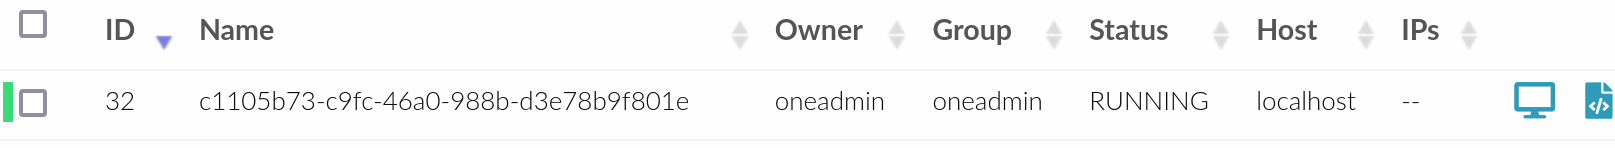
\includegraphics[width=\textwidth]{tesi_screenshot/OpenNebula_firstVM.png}
        \caption{Dashboard di OpenNebula con una sola virtual machine}
    \end{minipage}
    \begin{minipage}{0.49\textwidth}
        \centering
        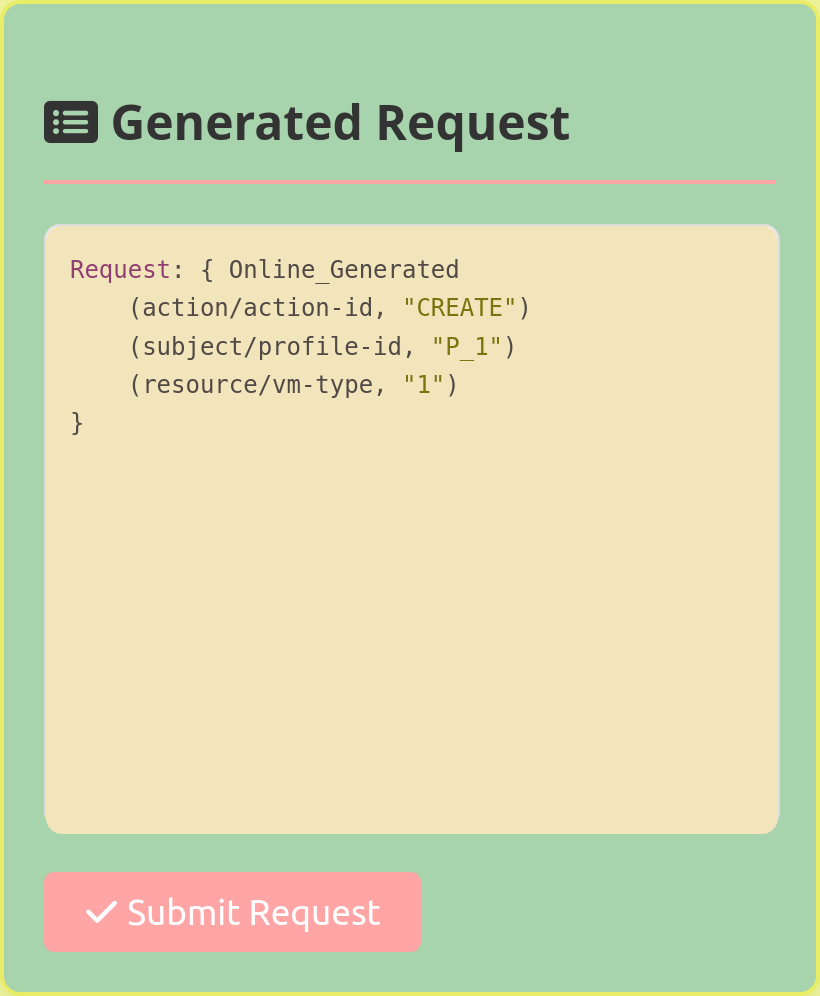
\includegraphics[width=\textwidth]{tesi_screenshot/P1Create_1.png}
    \end{minipage}
    \begin{minipage}{0.49\textwidth}
        \centering
        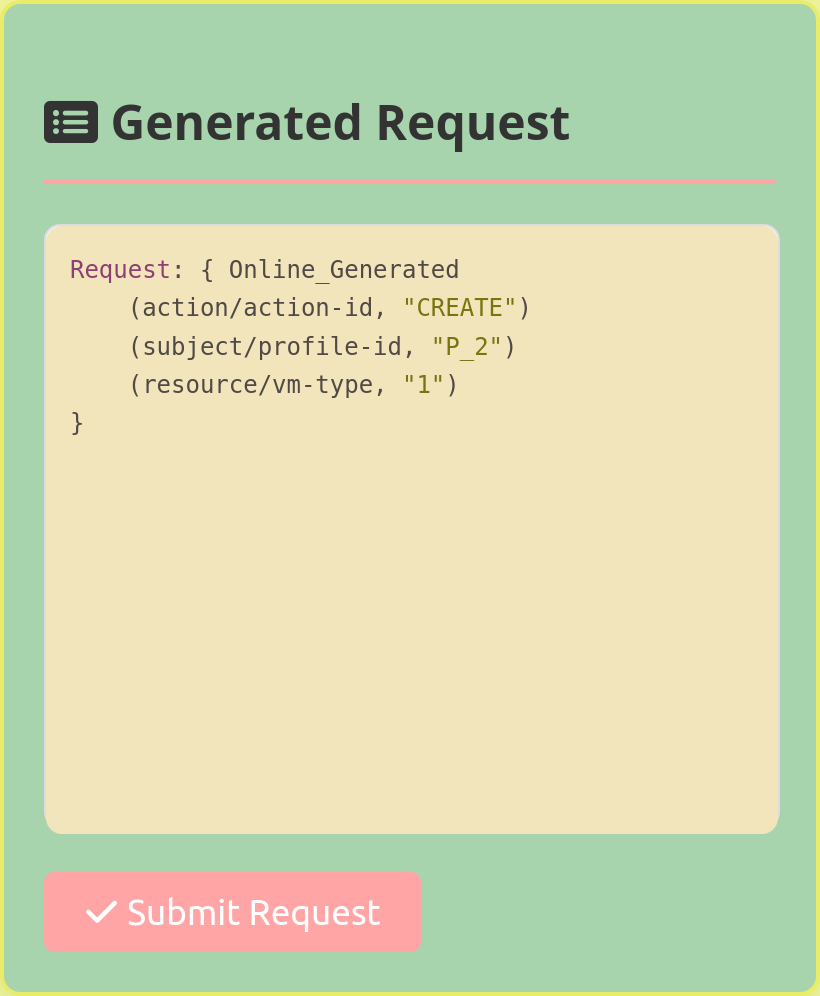
\includegraphics[width=\textwidth]{tesi_screenshot/P2Create_1.png}
    \end{minipage}
    \caption{Richieste di P\_1 e P\_2}
\end{figure}
Come si può vedere nonostante siano state eseguite due richieste è stata creata soltanto una macchina virtuale. Questa logica è corretta perchè l'utente P\_1 non è autorizzato a creare virtual machine con il template 1. Le valutazione del sistema FACPL sono quindi:
\begin{figure}[H]
    \begin{minipage}{0.27\textwidth}
        \centering
        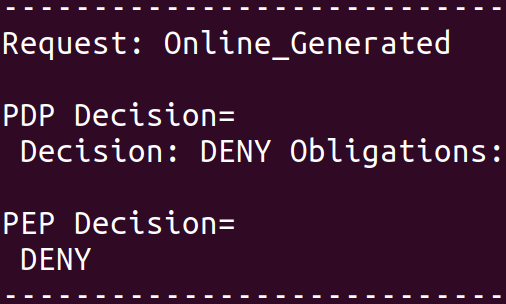
\includegraphics[width=\textwidth]{tesi_screenshot/DenyP1_1_cut.png}
    \end{minipage}
    \begin{minipage}{0.72\textwidth}
        \centering
        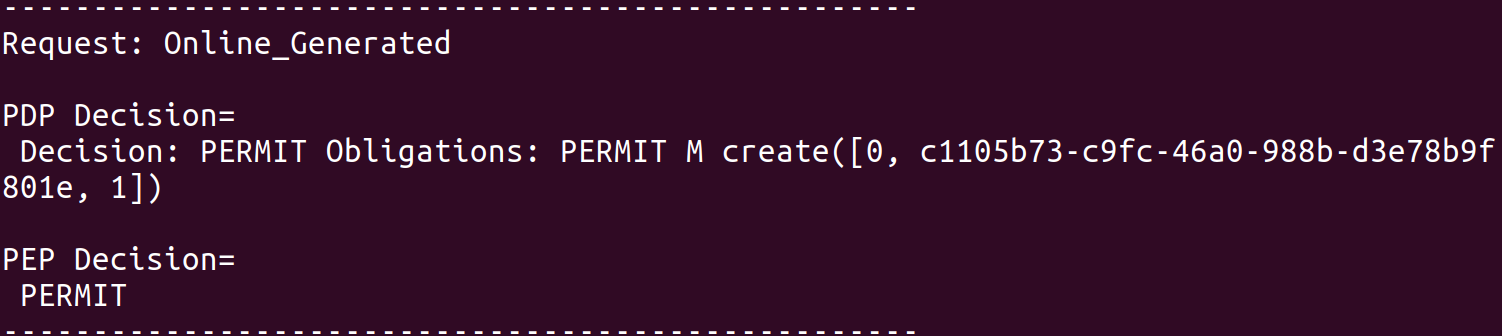
\includegraphics[width=\textwidth]{tesi_screenshot/Permit_P2_1.png}
    \end{minipage}
    \caption{Valutazioni di FACPL sulle due richieste}
\end{figure}
A questo punto sono state inviate ulteriori richieste da utenti con \emph{ID} P\_2 sia per virtual machine di tipo 1 che per virtual machine di tipo 0. Si nota che il sistema continua ad inserire tutte le virtual machine sul \emph{server} fino a che non si raggiunge un bilanciamento di risorse rimaste tra \emph{server} e \emph{laptop}:
\begin{figure}[H]
    \centering
    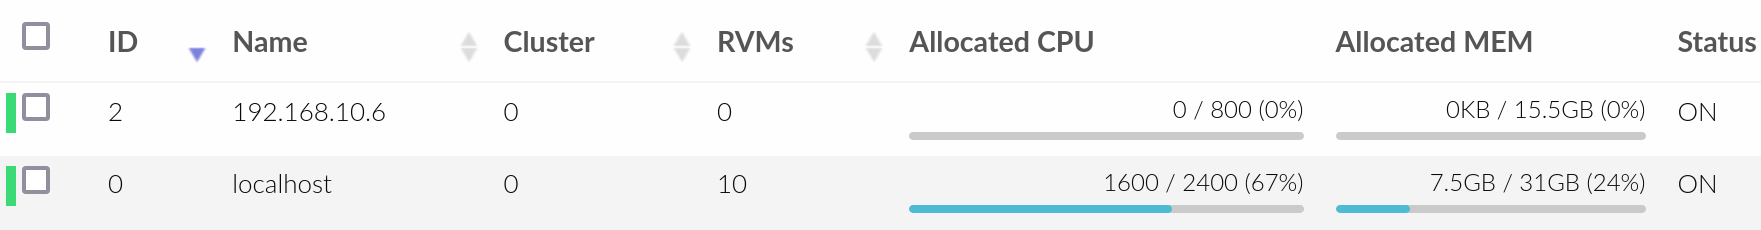
\includegraphics[width=\textwidth]{tesi_screenshot/OpenNebula_eavenLoad.png}
    \caption{Dashboard di OpenNebula con i due host bilanciati}
\end{figure}
Il load balancing sembra quindi funzionare correttamente. Per mostrarlo ulteriormente si continuano a creare delle virtual machine di modo da verificare che comincino ad essere aggiunte anche all'interno del \emph{laptop}:
\begin{figure}[H]
    \centering
    \includegraphics[width=\textwidth]{tesi_screenshot/alternating.png}
    \caption{Dashboard con le virtual machine alternate fra i due host}
\end{figure}
Continuando in questo modo si raggiunge una situazione in cui entrambi gli host hanno tutte le CPU utilizzate al 100\%. A questo punto secondo le policy scelte il sistema dovrebbe controllare se ci sono alcune virtual machine di tipo 1 da freezzare in favore della creazione di virtual machine di tipo 2. Questo infatti è quello che succede:
\begin{figure}[H]
    \centering
    \begin{minipage}{\textwidth}
        \centering
        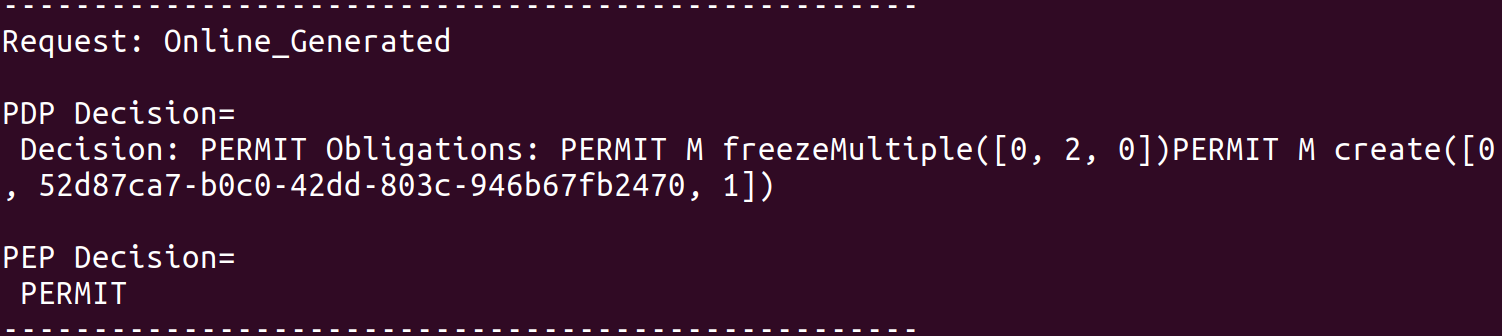
\includegraphics[width=\textwidth]{tesi_screenshot/permitReleaseCreateLonger.png}
        \caption{Valutazione di FACPL}
        \label{fig:full_hosts}
    \end{minipage}
    \begin{minipage}{\textwidth}
        \centering
        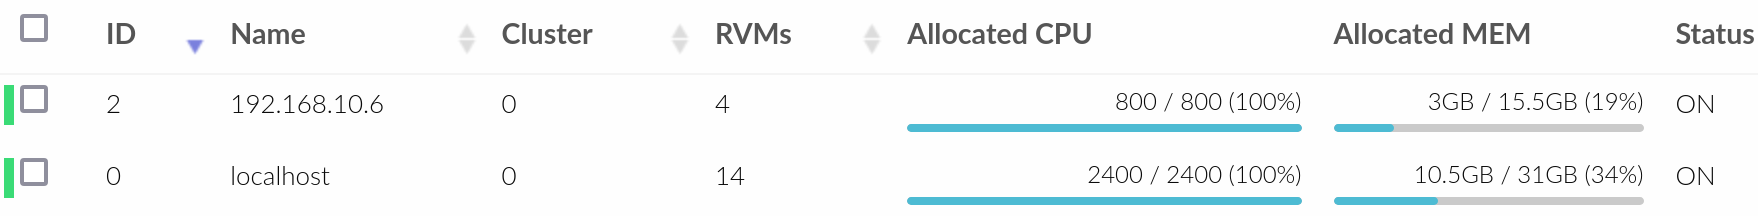
\includegraphics[width=\textwidth]{tesi_screenshot/full_hosts.png}
        \caption{Dashboard con entrambi gli host al 100\% di utilizzo}
        \label{fig:full_hosts}
    \end{minipage}
    \par \medskip
    \begin{minipage}{\textwidth}
        \centering
        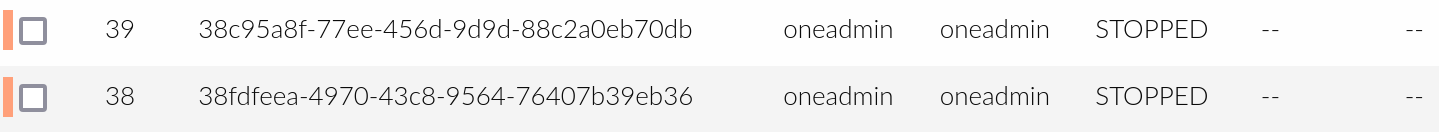
\includegraphics[width=\textwidth]{tesi_screenshot/stoppedVMS.png}
        \caption{virtual machine stoppate automaticamente}
    \end{minipage}
\end{figure}
Le due virtual machine freezzate erano appartenenti al \emph{server}, anche perchè era l'unico dei due host ad avere macchine di tipo 1 attive e quindi freezzabili. Possiamo notare questo anche nella figura \ref{fig:full_hosts}, dato che il numero delle virtual machine sul \emph{server} è 14. Questo numero è dato dalla presenza di 10 virtual machine che richiedono 2 processori l'una e 4 virtual machine che richiedono 1 processore l'una. Sul \emph{laptop} ci sono invece soltanto 4 virtual machine che richiedono 2 processori l'una.\par
Se si tenta di creare ulteriori virtual machine di tipo 1 il sistema FACPL ritorna correttamente una valutazione di \emph{DENY} e quindi la richiesta non viene neanche inviata a OpenNebula come si può vedere nella seguente immagine:
\begin{figure}[H]
    \centering
    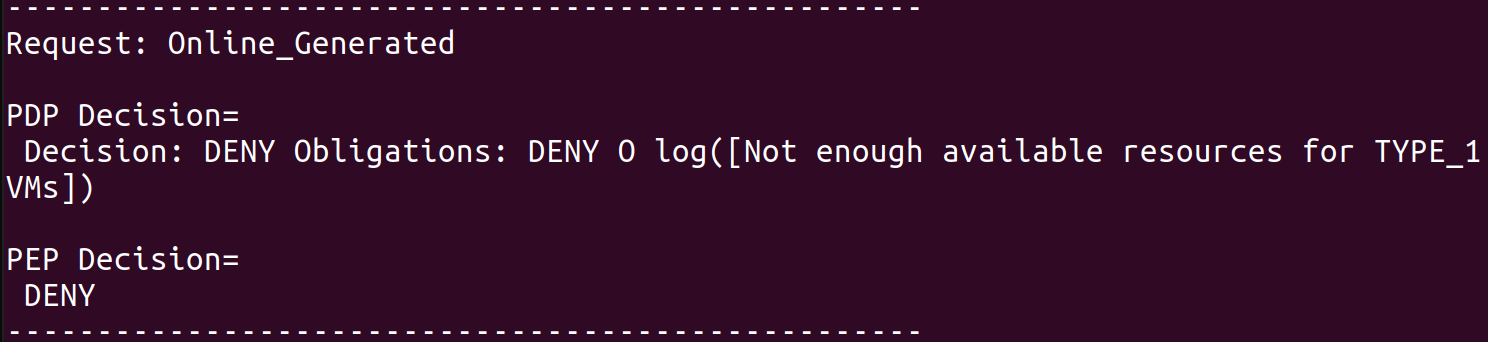
\includegraphics[width=\textwidth]{tesi_screenshot/notEnoughResources.png}
\end{figure}
Questo è un comportamento corretto dato che in realtà OpenNebula permette di sovraccaricare il sistema ma non è quello che vogliamo nel nostro caso.\par

A questo punto l'unico passo rimasto è testare se le macchine vengono correttamente rilasciate anche con l'utilizzo diretto delle richieste di tipo \emph{RELEASE}. Per fare questo si è resettato il sistema, si è poi creato una virtual machine e si è verificato che FACPL valutasse correttamente la richiesta di rilascio della stessa. Come si può vedere nelle seguenti figure l'esecuzione è andata a buon fine:
\begin{figure}[H]
    \centering
    \begin{minipage}{.5\textwidth}
        \centering
        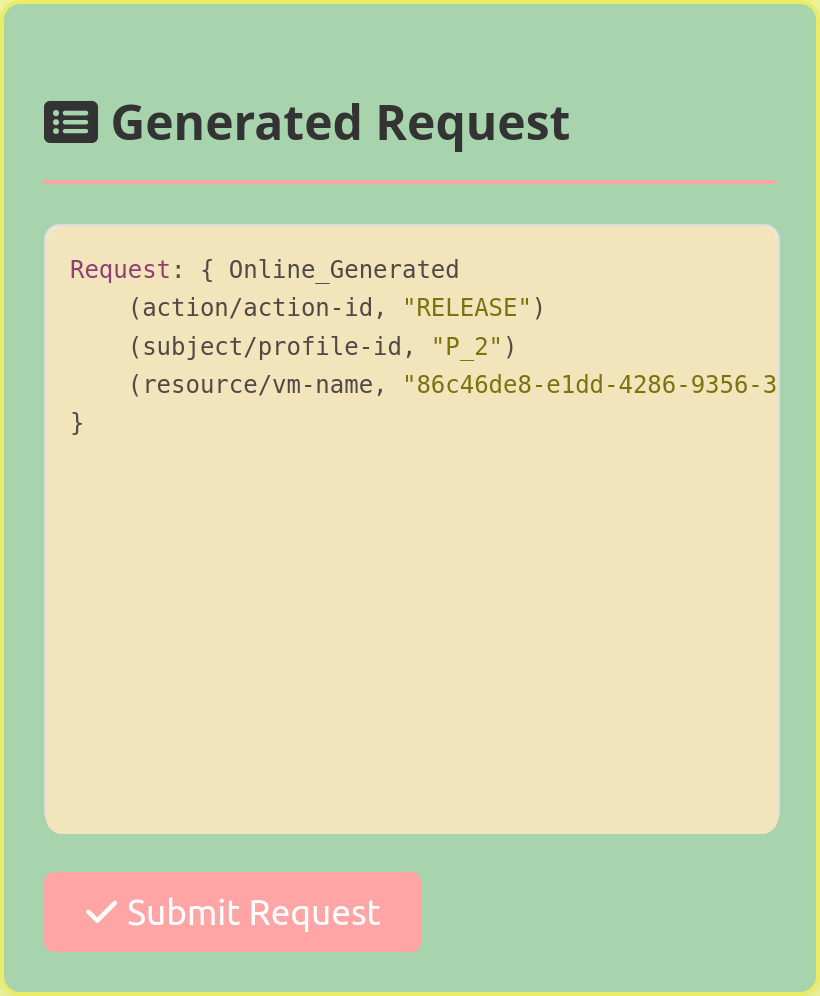
\includegraphics[width=\textwidth]{tesi_screenshot/ReleaseP2.png}
        \caption{Richiesta di rilascio}
    \end{minipage}
    \begin{minipage}{\textwidth}
        \centering
        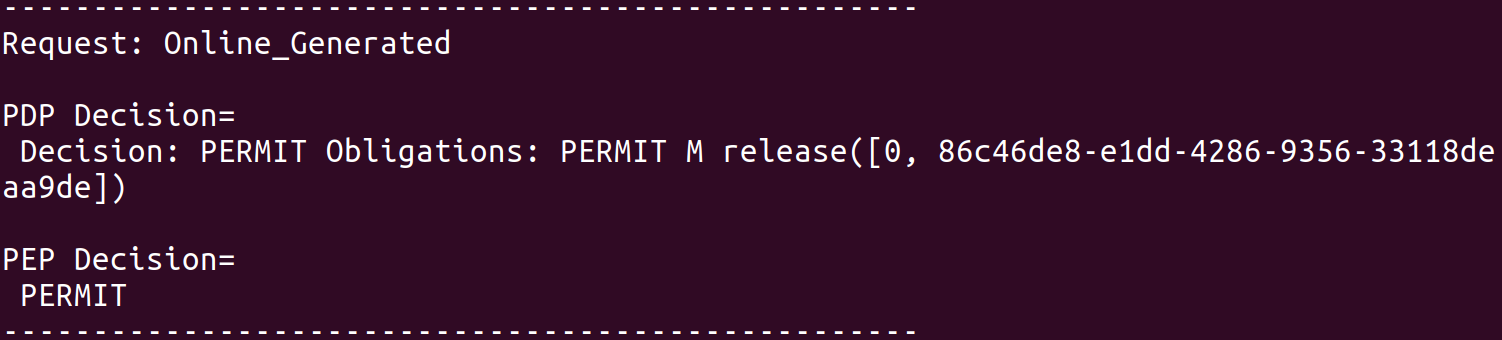
\includegraphics[width=\textwidth]{tesi_screenshot/permitRelease.png}
        \caption{valutazione di FACPL}
    \end{minipage}
    \par \medbreak
    \begin{minipage}{\textwidth}
        \centering
        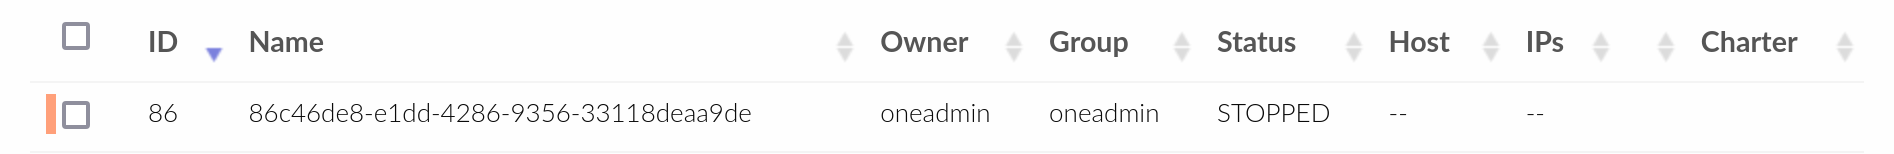
\includegraphics[width=\textwidth]{tesi_screenshot/stoppedVM.png}
        \caption{Virtual machine stoppata}
    \end{minipage}
\end{figure}
% !TEX root = ../Thesis.tex

\chapter{Conclusioni e sviluppi futuri}
In questo capitolo verranno analizzati i punti positivi e le criticità riscontrabili nella modalità di utilizzo di FACPL per un progetto come quello in esame. Ci si concentrerà quindi sui pregi e difetti che caratterizzano la libreria Java con cui viene distribuito. Saranno inoltre proposti alcuni sviluppi futuri per migliorare la libreria e anche per sviluppare ulteriormente i progetti ideati in questa tesi.

\section{Criticità e punti di forza della libreria Java di FACPL}
Per questo progetto le prime criticità sono state quelle riguardanti la poca diffusione di FACPL e la conseguente mancanza di documentazione molto dettagliata. Capire il funzionamento della libreria non è stato immediato dato che anche la documentazione ufficiale non è completa. Non è spiegato all'effettivo come implementare le componenti del sistema che devono per forza essere modificate a mano come mostrato nella sezione \ref{sec:modalitaFACPL}.\par
È anche vero però che una volta compreso come interagiscono fra loro le classi della libreria, inserire le funzionalità già sviluppate è stato molto semplice. Questo ci porta a considerare che in effetti la libreria è ben sviluppata ma manca soltanto di una documentazione un po' più specifica che indichi come integrare il software in un progetto più ampio; in particolar modo servirebbe una guida su come gestire le variabili di sistema e le \emph{PEPAction}.\par
Un'altra mancanza è una modalità semplice di conversione delle policy e delle richieste scritte in FACPL in codice Java. Sono documentati dei validatori e convertitori del linguaggio FACPL che però, come indicato più volte anche in questa tesi, sono utilizzabili tramite la UI di Eclipse. Nella libreria sono presenti delle classi di validazione e conversione di file da FACPL verso diversi linguaggi fra cui anche Java, tuttavia non è presente alcun tipo di documentazione al riguardo; guardando la letteratura si fa sempre riferimento ai convertitori automatici accessibili da Eclipse. Una strada percorribile molto facilmente per migliorare questo aspetto, sarebbe quella di consigliare l'utilizzo dello \emph{StandaloneGenerator} fornito come esempio.\par
Un altro aspetto migliorabile è la gestione delle dipendenze, usare un gestore come Maven renderebbe la libreria più appetibile per un utilizzatore e permetterebbe di rendere la libreria più mantenibile e più semplice da aggiornare.\par
L'ultima problematica riguarda la dipendenza da Java 8, in realtà questo problema è facilmente risolvibile. Ad esempio durante il nostro  sviluppo per un periodo si è compilato il codice con Java 11 senza problemi con qualche piccolo accorgimento. Tuttavia per evitare di dover svolgere test estensivi su parti di codice già testate con Java 8 si è dovuto ritornare ad utilizzare questa versione.\par
Parlando degli aspetti positivi troviamo sicuramente la facilità di integrazione con un progetto già esistente. Quando si utilizza FACPL un approccio che funziona bene è quello di pensare alla logica della propria implementazione in modo del tutto distaccato da FACPL e poi integrare le due parti. Per farlo basta scrivere del codice che fornisca due cose:
\begin{itemize}
    \item Dei metodi in grado di ritornare delle informazioni sullo stato del sistema
    \item Delle classi che permettano di eseguire delle azioni sul sistema e che devono aderire all'interfaccia \texttt{IPepAction}
\end{itemize}
A quel punto cambiando le classi \texttt{ContextStub\_Default} e \texttt{PepAction}, in poche righe il proprio codice è utilizzabile dal sistema FACPL.\par
L'altro aspetto molto positivo è la gestione del logging, infatti questo è già molto espressivo e permette di capire in modo dettagliato le scelte che vengono fatte dal sistema. Questo torna utile in fase di test del proprio codice, oltre che per un eventuale utilizzatore finale.\par

\section{Sviluppi futuri}
Per quanto riguarda la libreria Java di FACPL uno sviluppo futuro potrebbe riguardare l'aggiornamento ad una versione di Java LTS più recente come la 11 o la 17. Questo permetterebbe innanzitutto di rimuovere alcune dipendenze da librerie esterne, che sono entrare a far parte delle librerie standard nelle versioni più recenti di Java. Inoltre renderebbe la libreria più adatta ad essere integrata con codice più recente.\par
L'altro aspetto già largamente discusso sarebbe una nuova modalità di gestione delle dipendenze, che renderebbe sicuramente più facile anche eseguire il passo descritto sopra.\par
Per concludere, una volta aggiornata la libreria, sarebbe utile migliorare la documentazione e mostrare un workflow consigliato da seguire in dei progetti più grandi come quello considerato in questa tesi.\par
Per quanto riguarda invece i due progetti ideati in questa tesi, sicuramente ci sono diverse possibilità di ampliazione. Si potrebbe pensare di integrare molte più \emph{PEPAction} riguardanti OpenNebula. Questo passo non sarebbe difficile da fare dato che è già presente la classe astratta che può essere estesa e da cui partire per scrivere nuovi comandi. Alcuni comandi interessanti che potrebbero essere aggiunti sono il cambiamento di rete per una virtual machine o il cambiamento delle impostazioni di una virtual machine a runtime, entrambe azioni facilmente implementabili con le API di OpenNebula.\par

Una miglioria che si potrebbe portare avanti riguarda il front-end e l'integrazione di un sistema di autenticazione. Questa parte nella logica attuale è rimandata alla persona che intende inserire il codice nella sua infrastruttura. Il sistema di autenticazione potrebbe tornare utile per un utilizzatore finale che vuole partire da zero. Si considera però che nella maggior parte dei sistemi la nostra web-app sarà gestita tramite un sistema di autenticazione generale, che racchiude anche altre web-app. Il front-end è sicuramente migliorabile anche in molti altri modi, espressi nel capitolo \ref{cap:capitolo3}.\par
% !TEX root = ../Thesis.tex
\chapter*{Ringraziamenti}
\addcontentsline{toc}{chapter}{Ringraziamenti}



%--------------------------------------------------------------
% Bibliography
%--------------------------------------------------------------
\bibliographystyle{plain}
\phantomsection
\bibliography{Bibliography} % Entries are in the Bibliography.bib file

%--------------------------------------------------------------
\end{document}
%--------------------------------------------------------------
